\textbf{Глава 3} посвящена обнаруженному в работе механизму поддержания продольных вихрей. В \textbf{разделах 3.1 -- 3.3} механизм дается на примере решения, имеющего вид бегущей волны. Это решение периодично вдоль потока и стационарно в сопутствующей системе отсчета. Простота его поведения позволяет в более строгой форме показать ряд особенностей движения, обеспечивающих работу механизма. 

В \textbf{разделе 3.4} проводится обобщение механизма поддержания продольных вихрей на модельный порыв. 
Прояснить процесс поддержания продольных вихрей позволяет анализ уравнения эволюции средней продольной завихренности
\begin{multline}\label{OX_eq}
\pd{\Omega_x}{t} + (V_x - c_f)\pd{\Omega_x}{x} + V_r \pd{\Omega_x}{r} + \frac{V_\theta}{r} \pd{\Omega_x}{\theta} - \nu\nabla^2\Omega_x= \Omega_x \pd{V_x}{x} + \Omega_r \pd{V_x}{r} + \\ + \frac{\Omega_\theta}{r} \pd{V_x}{\theta}
 - \overline{v'_x \pd{\omega'_x}{x}}^t - \overline{v'_r \pd{\omega'_x}{r}}^t - \overline{\frac{v'_\theta}{r} \pd{\omega'_x}{\theta}}^t
 + \overline{\omega'_x \pd{v'_x}{x}}^t + \overline{\omega'_r \pd{v'_x}{r}}^t + \overline{\frac{\omega'_\theta}{r} \pd{v'_x}{\theta}}^t,
\end{multline}
в котором $\Om = (\Omega_x, \Omega_r, \Omega_\theta)$ и $\om' = (\omega'_x, \omega'_r, \omega'_\theta)$ --- средняя и пульсационная составляющие вектора завихренности $\om = \rot \v$, $c_f$ --- скорость перемещения системы отсчета. Система находится в равновесии и средняя завихренность во времени не меняется. Источниковые слагаемые в правой части уравнения компенсируются конвективными и вязкими слагаемыми в левой. Анализ уравнения \eqref{OX_eq} показал, что два слагаемых в правой части, а именно
\begin{equation}\label{OXgen_terms}
- \overline{v'_x \frac{\d \omega'_x}{\d x}}^t + \overline{ \omega'_x \frac{\d v'_x}{\d x} }^t,
\end{equation}
вносят определяющий вклад в производство средней продольной завихренности. 

Для представления количественных данных обратимся к уравнения эволюции квадрата $\Omega_x$, полученному умножением \eqref{OX_eq} на $2\Omega_x$. Положительный или отрицательный знак у выражений в правой части этого уравнения показывает соответственно положительный или отрицательный вклад этого члена в изменение $\Omega^2_x$, а следовательно, и в интенсивность поперечного движения. Распределение $\Omega^2_x$ по сечению трубы представлено на рисунке \ref{OXgen_pic}(a). Область концентрации $\Omega_x$ расположена между полосами повышенной и пониженной скорости вблизи области максимальной амплитуды пульсаций. Соответствующее сумме \eqref{OXgen_terms} распределение в уравнении для $\Omega^2_x$ представлено на рисунке \ref{OXgen_pic}(б), а вклад остальных слагаемых правой части \eqref{OX_eq} показан на рисунке \ref{OXgen_pic}(в). Распределение генерации $\Omega^2_x$ выделенными в \eqref{OXgen_terms} членами практически совпадает по форме с распределением $\Omega^2_x$, тогда как вклад остальных членов не имеет выраженного распределения и более чем на порядок уступает по суммарному вкладу в генерацию $\Omega^2_x$. Таким образом, нет сомнения в том, что стационарные продольные вихри возникают за счет действия слагаемых \eqref{OXgen_terms}.

\begin{figure}
\center{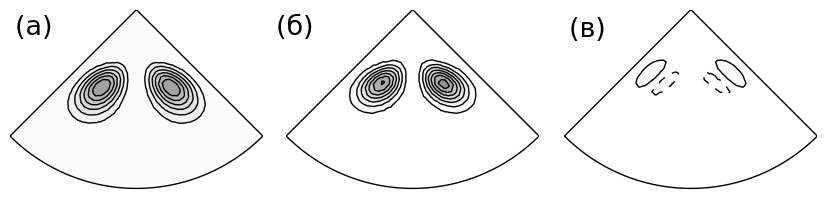
\includegraphics[width=1\linewidth]{autoref_OXgen.png}}
\caption{Механизм генерации продольных вихрей}
\label{OXgen_pic}
\end{figure}

Между собой слагаемые \eqref{OXgen_terms} практически равны. Это значит, в частности, что колебания $\partial v'_x / \partial x$ и $\omega'_x$ положительно коррелированы в области концентрации положительной $\Omega_x$ и отрицательно коррелированы в области концентрации отрицательной $\Omega_x$. То же относится и к колебаниям $-v'_x$ и $\partial \omega'_x / \partial x$. Выявить механизм формирования такой связи позволяет анализ уравнения эволюции $\omega'_x$:
\begin{multline}\label{ox1_eq}
\pd{\omega'_x}{t} + (V_x - c_\mathrm{tw})\pd{\omega'_x}{x} + V_r \pd{\omega_x'}{r} + \frac{V_\theta}{r} \pd{\omega'_x}{\theta} 
- \nu\nabla^2\omega'_x = - v'_x \pd{\Omega_x}{x} - v'_r \pd{\Omega_x}{r} - \\ - \frac{v'_\theta}{r} \pd{\Omega_x}{\theta} 
+ \Omega_x \pd{v'_x}{x} + \Omega_r \pd{v'_x}{r} + \frac{\Omega_\theta}{r} \pd{v'_x}{\theta}
+ \omega'_x \pd{V_x}{x} + \omega'_r \pd{V_x}{r} + \frac{\omega'_\theta}{r} \pd{V_x}{\theta} - \\ 
- v'_x \pd{\omega'_x}{x} - v'_r \pd{\omega'_x}{r} - \frac{v'_\theta}{r} \pd{\omega'_x}{\theta} 
+ \omega'_x \pd{v'_x}{x} + \omega'_r \pd{v'_x}{r} + \frac{\omega'_\theta}{r} \pd{v'_x}{\theta} + \\
+ \overline{v'_x \pd{\omega'_x}{x}}^t + \overline{v'_r \pd{\omega'_x}{r}}^t + \overline{\frac{v'_\theta}{r} \pd{\omega'_x}{\theta}}^t
- \overline{\omega'_x \pd{v'_x}{x}}^t - \overline{\omega'_r \pd{v'_x}{r}}^t - \overline{\frac{\omega'_\theta}{r} \pd{v'_x}{\theta}}^t.
\end{multline}
%Умножение \eqref{ox1_eq} на $2\omega'_x$ и последующее осреднение по времени дает уравнение баланса среднего квадрата пульсаций продольной завихренности $\overline{\omega'_x\omega'_x}^t$. Слагаемые в этом уравнении не зависят от времени. Как и в предыдущем случае, с
Среди всех источниковых слагаемых в правой части \eqref{ox1_eq} также удалось выделить существенные, ответственные за возникновение пульсаций $\omega'_x$. Как показано в работе, в области формирования продольных вихрей за образование $\omega'_x$ отвечает слагаемое
\begin{equation}\label{ox1gen_main_terms}
\frac{\d \omega'_x}{\d t} = \Omega_x \frac {\d v'_x}{\d x} + ...
\end{equation}
Выделенное в \eqref{ox1gen_main_terms} слагаемое отвечает за перераспределение уже существующей стационарной продольной завихренности $\Omega_x$ пульсационной составляющей продольной скорости $v'_x$ (эффект сжатия/растяжения вихревых трубок). Оно стремится произвести пульсации $\omega'_x$, пропорциональные $\d v'_x / \d x$, причем коэффициентом пропорциональности выступает средняя продольная завихренность. Соответственно, механизм включается в областях концентрации~$\Omega_x$. В области расположения положительного вихря производимые пульсации $\omega'_x$ положительно пропорциональны пульсациям $\d v'_x / \d x$, а в области расположения отрицательного вихря --- отрицательно пропорциональны. Таким образом обеспечивается максимально возможная эффективность производства средней продольной завихренности нужного знака посредством второго из слагаемых \eqref{OXgen_terms}. Пульсации $-v'_x$ и $\d \omega'_x / \d x$ отказываются также согласованы нужным образом, и первое слагаемое \eqref{OXgen_terms} оказывается равно второму.

Фазовая скорость бегущей волны, соответствующей пульсационной составляющей движения, совпадает со средней скоростью жидкости в области формирования продольных вихрей. По этой причине формируемые \eqref{ox1gen_main_terms} пульсации $\omega'_x$, перемещаясь вниз по потоку за счет конвекции, остаются в фазе с порождающими их пульсациями $\partial v'_x / \partial x$.

В \textbf{разделе 3.5} приведены выводы по главе. Основные результаты главы опубликованы в работах автора диссертации \cite{MZG2017,  KMU17}.

 
